% !TEX TS-program = xelatex
% !TEX encoding = UTF-8
% !Mode:: "TeX:UTF-8"

\documentclass[onecolumn,oneside]{BUPTHomework}

\usepackage{blindtext}

\author{胡玉斌}
\sid{202111054}
\title{第一章\ 作业题}
\coursecode{3131100063}
\coursename{编码理论}

\begin{document}
  \maketitle
  
  \begin{problem}[5]
  {
    考虑表1.1中列出的信源符号和它们相应的概率。
    对于这个码,求信源的熵、每个符号的平均二元字节数、该码的效率。

    \begin{table}[!htbp]
      \centering
      \begin{tabular}{|c|c|c|c|}
      \hline
      符号    & 概率   & 自信息    & 码字 \\ \hline
      $x_1$ & 0.40 & 1.3219 & 1  \\ \hline
      $x_2$ & 0.35 & 1.5146 & 00 \\ \hline
      $x_3$ & 0.25 & 2.0000 & 01 \\ \hline
      \end{tabular}
      \caption{信源符号和它们相应的概率、自信息及码字}
    \end{table}
  }
  \end{problem}

  \begin{solution}
  {
    \textbf{\textsf{信源的熵:}}
    
    \begin{eqnarray} 
      H(X) &=& -\sum_{i=1}^{3}P(x_i)\log_2 P(x_i) \nonumber \\
      &=& -x_1\log_2 (x_1)-x_2\log_2 (x_2)-x_3\log_2 (x_3) \nonumber \\
      &=& 0.40\times \log_2 (\frac{1}{0.4})+0.35\times \log_2 (\frac{1}{0.35})+0.25\times \log_2 (\frac{1}{0.25}) \nonumber \\
      &=& 1.5589\ \mbox{(bit)} \nonumber
    \end{eqnarray}

    \textbf{\textsf{每个符号的平均二元字节数:}}

    \begin{eqnarray} 
      \overline{R} &=& \sum_{i=1}^{3}n_iP(x_i) \nonumber \\
      &=& 1 \times 0.40 + 2 \times 0.35 + 2 \times 0.25 \nonumber \\
      &=& 1.60\ \mbox{(bit)} \nonumber
    \end{eqnarray}

    \textbf{\textsf{该码的效率:}}

    \begin{eqnarray} 
      R &=& \frac{H(U)}{\overline{R}} \nonumber \\
      &=& \frac{1.5589}{1.60} \nonumber \\
      &=& 0.9743 \nonumber
    \end{eqnarray}
  }
  \end{solution}


  \begin{problem}[12]
  {
    为什么要用信道编码器?信道编码要满足什么定理?请给出该定理的内容。
  }
  \end{problem}

  \begin{solution}
  {
    为了使传输有效。
    信道编码器将信息序列 $U$ 变换成离散的有结构的编码序列 $X$,这称为码字。
    即为了使传输有效,人为的增加一些冗余度,使其具有自动检错和纠错的能力。
    码字的结构主要用以对付传输或储存码字的有扰信道。

    信道编码要满足信道编码定理(仙农第二定理)。
    信道编码定理是阐明使传信率逼近信道容量大编码是存在的定律。
    如果系统的传输率小于信道容量,那么适当选择编码技术就能实现可靠通信,即可以将差错率减小到任意小的程度。
    每个信道都具有固定的信道容量 $C$ ,对任何小于 $C$ 对信息传输率 $R$ ,存在一个码长为 $n$ 码率为 $R$ 对分组码。
    若用最大似然译码,则其译码错误概率为  $P_e \leq \land e^{-nE_b(R)}$  。
    对于码率为 $R$ 约束长度为 $n_e$ 对卷积码,其译码错误概率也有类似的关系。
    其中 $A$ 和 $B$ 都为大于0对数, $E_b(R)$ 和  $E_e(R)$ 为正实函数,叫做误差函数。 
  }
  \end{solution}


  \begin{problem}[18]
  {
    对于如图3.1所示的BSC信道,信源符号发生的概率为 $P(x_1)=0.6,P(x_2)=0.4$ 。求:
    \begin{enumerate}
      \item 信源 $X$ 中事件 $x_1$ 和 $x_2$ 分别的自信息(以比特为单位);
      \item 接收符号 $y_i(i=1,2)$ 发生的概率;
      \item 求条件概率 $P(x_i \vert y_i)$ ;
      \item 收到消息 $y_i(i=1,2)$ 后,获得的关于 $x_i(i=1,2)$ 的信息量;
      \item 信源 $X$ 和信源 $Y$ 的信息熵;
      \item 条件熵 $H(X \vert Y)$ 和 $H(Y \vert X)$。
    \end{enumerate}

    \begin{figure}[!htbp]
      \centering
      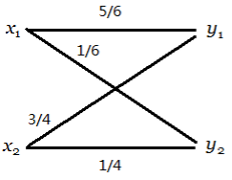
\includegraphics[width = 4cm ]{image/picture1.png}
      \caption{二元BSC信道}
    \end{figure}
  }
  \end{problem}

  \begin{solution}
  {
    \begin{enumerate}
      \item 信源 $X$ 中事件 $x_1$ 和 $x_2$ 分别的自信息(以比特为单位);
      
      \begin{eqnarray} 
        I(x_1) &=& \log \frac{1}{P(x_1)} = \log \frac{1}{0.6} = 0.737\ \mbox{(bit)} \nonumber
      \end{eqnarray}
      
      \begin{eqnarray} 
        I(x_2) &=& \log \frac{1}{P(x_2)} = \log \frac{1}{0.4} = 1.322\ \mbox{(bit)} \nonumber
      \end{eqnarray}

      \item 接收符号 $y_i(i=1,2)$ 发生的概率;
      
      \begin{eqnarray} 
        P(y_1) &=& P(x_1) \times P(y_1 \vert x_1) + P(x_2) \times P(y_2 \vert x_1) \nonumber \\
        &=& 0.6 \times \frac{5}{6} + 0.4 \times \frac{3}{4} \nonumber \\
        &=& 0.8 \nonumber
      \end{eqnarray}

      \begin{eqnarray} 
        P(y_2) &=& P(x_1) \times P(y_1 \vert x_2) + P(x_2) \times P(y_2 \vert x_2) \nonumber \\
        &=& 0.6 \times \frac{1}{6} + 0.4 \times \frac{1}{4} \nonumber \\
        &=& 0.2 \nonumber 
      \end{eqnarray}

      \item 求条件概率 $P(x_i \vert y_i)$ ;
      
      \begin{eqnarray} 
        P(x_1 \vert y_1) &=& \frac{P(x_1)P(y_1 \vert x_1)}{\sum_{j=1}^2P(x_j)P(y_1 \vert x_j)} \nonumber \\
        &=& \frac{0.6 \times \frac{5}{6}}{0.6 \times \frac{5}{6} + 0.4 \times \frac{3}{4}} \nonumber \\
        &=& 0.625 \nonumber
      \end{eqnarray}

      \begin{eqnarray} 
        P(x_2 \vert y_1) &=& \frac{P(x_2)P(y_1 \vert x_2)}{\sum_{j=1}^2P(x_j)P(y_1 \vert x_j)} \nonumber \\
        &=& \frac{0.4 \times \frac{3}{4}}{0.6 \times \frac{5}{6} + 0.4 \times \frac{3}{4}} \nonumber \\
        &=& 0.375 \nonumber
      \end{eqnarray}

      \begin{eqnarray} 
        P(x_1 \vert y_2) &=& \frac{P(x_1)P(y_2 \vert x_1)}{\sum_{j=1}^2P(x_j)P(y_2 \vert x_j)} \nonumber \\
        &=& \frac{0.6 \times \frac{1}{6}}{0.6 \times \frac{1}{6} + 0.4 \times \frac{1}{4}} \nonumber \\
        &=& 0.5 \nonumber
      \end{eqnarray}

      \begin{eqnarray} 
        P(x_2 \vert y_2) &=& \frac{P(x_2)P(y_2 \vert x_2)}{\sum_{j=1}^2P(x_j)P(y_2 \vert x_j)} \nonumber \\
        &=& \frac{0.4 \times \frac{1}{4}}{0.6 \times \frac{1}{6} + 0.4 \times \frac{1}{4}} \nonumber \\
        &=& 0.5 \nonumber
      \end{eqnarray}
      
      \item 收到消息 $y_i(i=1,2)$ 后,获得的关于 $x_i(i=1,2)$ 的信息量;
      
      \begin{eqnarray} 
        I(x_1 \vert y_1) &=& -\log_2P(x_1 \vert y_1) \nonumber \\
        &=& -\log_2(0.625) \nonumber \\
        &=& 0.67807\ \mbox{(bit)} \nonumber
      \end{eqnarray}
      
      \begin{eqnarray} 
        I(x_2 \vert y_1) &=& -\log_2P(x_2 \vert y_1) \nonumber \\
        &=& -\log_2(0.375) \nonumber \\
        &=& 1.41503\ \mbox{(bit)} \nonumber
      \end{eqnarray}

      \begin{eqnarray} 
        I(x_1 \vert y_2) &=& -\log_2P(x_1 \vert y_2) \nonumber \\
        &=& -\log_2(0.5) \nonumber \\
        &=& 1\ \mbox{(bit)} \nonumber
      \end{eqnarray}

      \begin{eqnarray} 
        I(x_2 \vert y_2) &=& -\log_2P(x_2 \vert y_2) \nonumber \\
        &=& -\log_2(0.5) \nonumber \\
        &=& 1\ \mbox{(bit)} \nonumber
      \end{eqnarray}

      \item 信源 $X$ 和信源 $Y$ 的信息熵;
      
      \begin{eqnarray}
        H(X) &=& - \sum_{i=1}^2P(x_i)\log_2 P(x_i) \nonumber \\
        &=& -0.6 \times \log_2(0.6) - 0.4 \times \log_2(0.4) \nonumber \\
        &=& 0.97095\ \mbox{(bit)}
      \end{eqnarray}

      \begin{eqnarray}
        H(Y) &=& - \sum_{i=1}^2P(y_i)\log_2 P(y_i) \nonumber \\
        &=& -0.8 \times \log_2(0.8) - 0.2 \times \log_2(0.2) \nonumber \\
        &=& 0.72193\ \mbox{(bit)}
      \end{eqnarray}
      
      \item 条件熵 $H(X \vert Y)$ 和 $H(Y \vert X)$。
      
      \begin{eqnarray}
        H(X \vert Y) &=& \sum_{i=1}^2\sum_{j=1}^2P(x_iy_j)\log_2 \frac{1}{P(x_i\vert y_j)} \nonumber \\
        &=& -\sum_{i=1}^2\sum_{j=1}^2P(x_i,y_j)\log_2 P(x_i\vert y_j) \nonumber \\
        &=& -0.8 \times 0.625 \times \log_2(0.625) - 0.8 \times 0.375 \times \log_2(0.375) - 0.2 \times 0.5 \times \log_2(0.5) - 0.2 \times 0.5 \times \log_2(0.5) \nonumber \\
        &=& 0.96355\ \mbox{(bit)} \nonumber 
      \end{eqnarray}

      \begin{eqnarray}
        H(Y \vert X) &=& \sum_{i=1}^2\sum_{j=1}^2P(y_ix_j)\log_2 \frac{1}{P(y_i\vert x_j)} \nonumber \\
        &=& -\sum_{i=1}^2\sum_{j=1}^2P(y_i,x_j)\log_2 P(y_i\vert x_j) \nonumber \\
        &=& - 0.6 \times \frac{5}{6} \times \log_2(\frac{5}{6}) - 0.6 \times \frac{1}{6} \times \log_2(\frac{1}{6}) - 0.4 \times \frac{3}{4} \times \log_2(\frac{3}{4}) - 0.4 \times \frac{1}{4} \times \log_2(\frac{1}{4}) \nonumber \\
        &=& 0.71452\ \mbox{(bit)} \nonumber 
      \end{eqnarray}
      
    \end{enumerate}
  }
  \end{solution}

  \begin{problem}[19]
  {
    上机题。
    \begin{enumerate}
      \item 如何编程序实现霍夫曼编码?
    \end{enumerate}
  }
  \end{problem}

  \begin{solution}
  {
    \textbf{\textsf{huffmanTree.h}}
\begin{lstlisting}
#include <iostream>
#include <queue>
#include <map>
#include <string>

using namespace std;

namespace HuffmanTree {

    struct Node{
        char c;
        int frequency;
        Node *left;
        Node *right;

        Node(char _c, int _frequency, Node *_left = nullptr, Node *_right = nullptr)
                : c(_c), frequency(_frequency), left(_left), right(_right) {}

        bool operator<(const Node &node) const {
            return frequency > node.frequency;
        }
    };

    class huffmanTree
    {
    private:
        std::priority_queue<Node> pq;

        void _huffmanCode(Node *node,
                          std::string &prefix,
                          std::map<char,
                          std::string>& codeMap) {
            std::string tmp = prefix;
            if (node->left != nullptr) {
                prefix += '0';
                if (_isLeaf(node->left)) {
                    codeMap[node->left->c] = prefix;
                } else {
                    _huffmanCode(node->left, prefix, codeMap);
                }
            }
            if (node->right != nullptr) {
                prefix = tmp;
                prefix += '1';
                if (_isLeaf(node->right)) {
                    codeMap[node->right->c] = prefix;
                } else {
                    _huffmanCode(node->right, prefix, codeMap);
                }
            }
        }

        static bool _isLeaf(Node* node) {
            return node->left == nullptr && node->right == nullptr;
        }

    public:
        huffmanTree(const std::map<char, int> alphabet) {
            for(auto x : alphabet) {
                Node node(x.first, x.second);
                pq.push(node);
            }
            genHuffmanTree();
        }
        ~huffmanTree() {

        }
        void genHuffmanTree() {
            while(pq.size() != 1) {
                Node *left = new Node(pq.top());
                pq.pop();
                Node *right = new Node(pq.top());
                pq.pop();
                Node node('.', left->frequency + right->frequency, left, right);
                pq.push(node);
            }
        }
        void huffmanCode(std::map<char, std::string> &codeMap) {
            Node node = pq.top();
            std::string prefix;
            _huffmanCode(&node, prefix, codeMap);
        }
    };
}
\end{lstlisting}

    \textbf{\textsf{main.cpp}}
\begin{lstlisting}
#include "huffmanTree.h"

using namespace HuffmanTree;

int main() {
    std::map<char, int> _alphabet = 
      {{'a', 5}, {'b', 4}, {'c', 3}, {'d', 2}, {'e', 1}};
    std::map<char, std::string> _codeMap;

    huffmanTree tree(_alphabet);
    tree.huffmanCode(_codeMap);

    for(auto x : _codeMap) {
        printf("%c: %s\n", x.first, x.second.c_str());
    }

    return 0;
}
\end{lstlisting}

    \textbf{\textsf{output:}}
    \begin{itemize}
      \item a: 11
      \item b: 10
      \item c: 00
      \item d: 011
      \item e: 010
    \end{itemize}

  }
  \end{solution}

\end{document}
